%!TEX root = ../my_thesis.tex
\section{Particle identification plots}
\label{app:pid}

The $p$ and $\eta$
distributions, as well as the $\PIDK$ efficiency and misidentification rates before the
resampling in bins of $p$ and $\eta$ are shown in Figs.~\ref{fig:PIDKeffPiBac}
and \ref{fig:PIDKeffKBac} for the bachelor particle of the signal, and in Fig.~\ref{fig:PIDKeffBac} for the $\Dmp$ daughters.
\begin{figure}[htpb]
	\begin{center}
		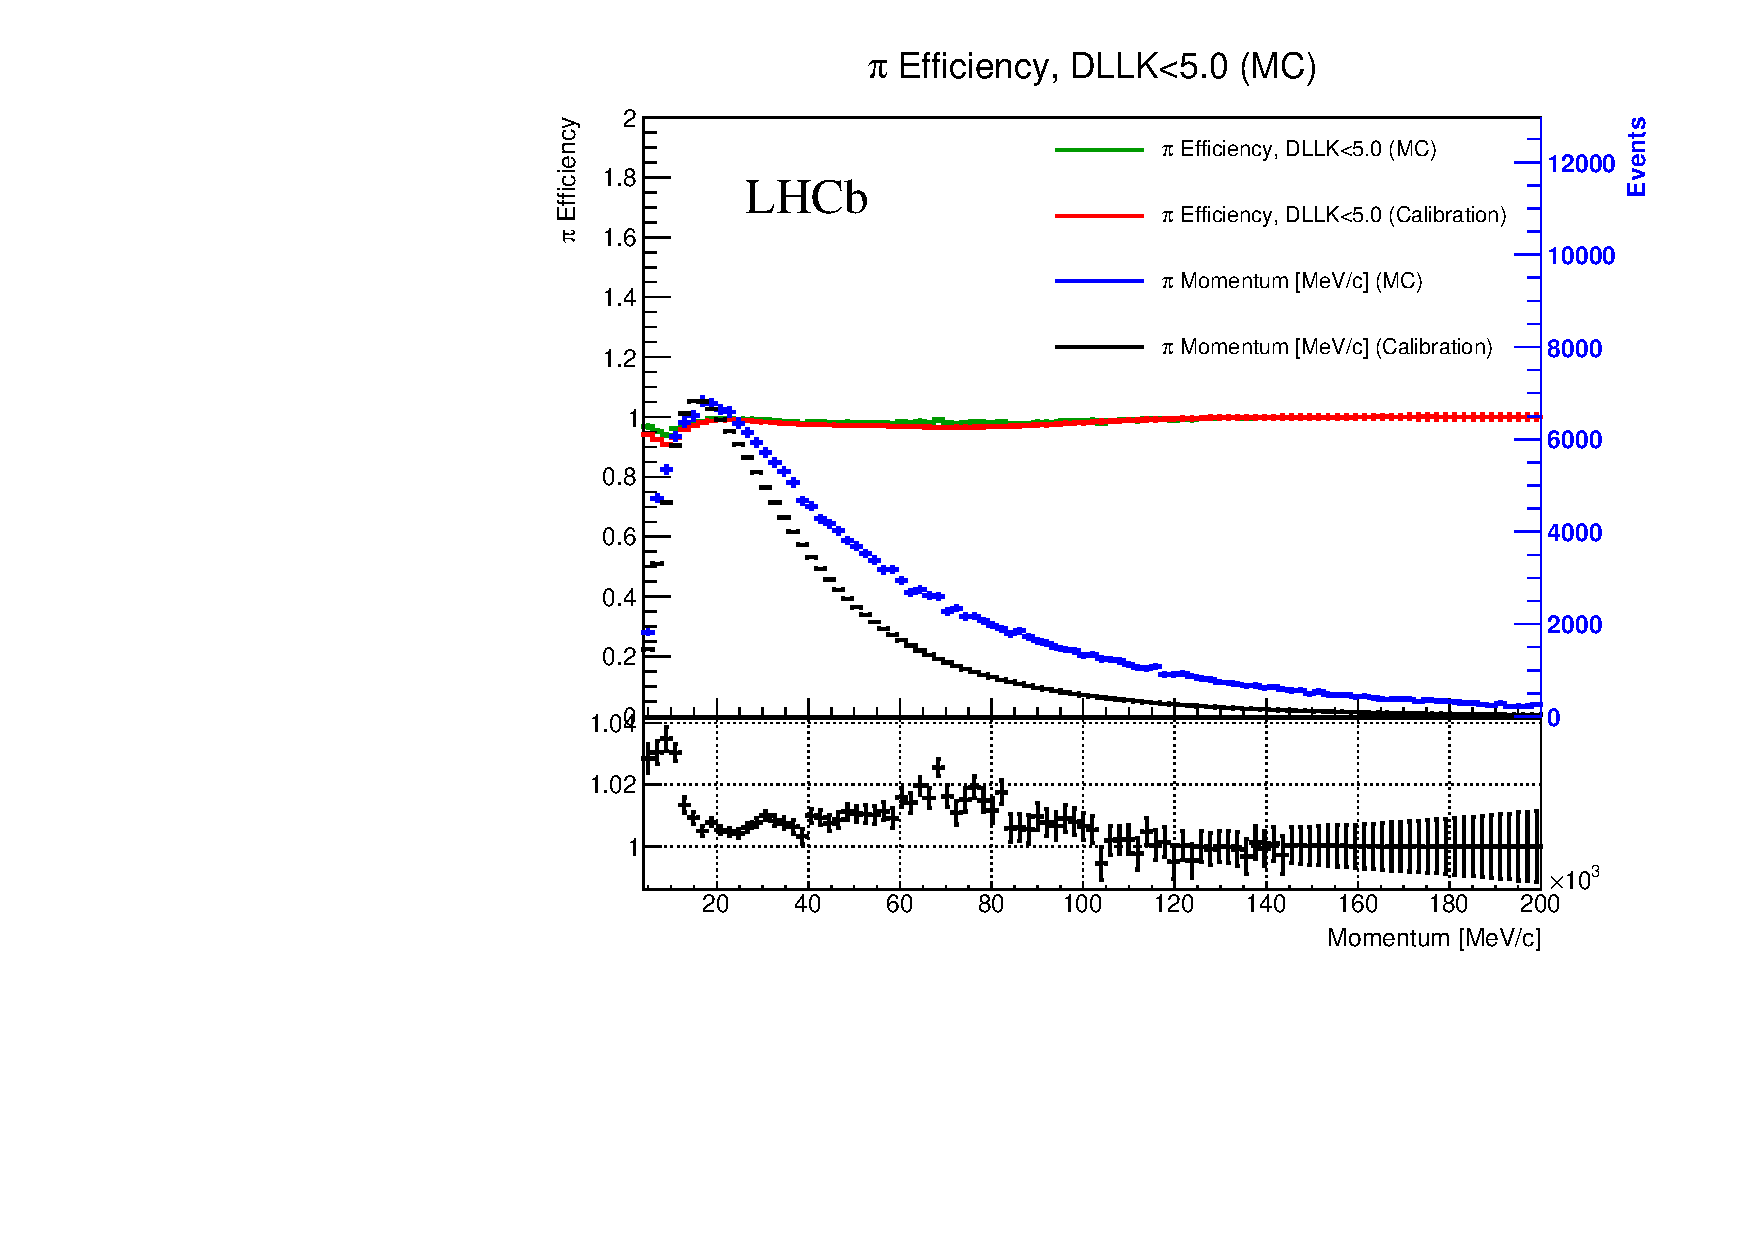
\includegraphics[width=0.495\linewidth]{AA-Appdx-pid/figs/Bd2DPi_BacPi_DLLKlt5_PIDeff_beforeResampling_P.pdf}
		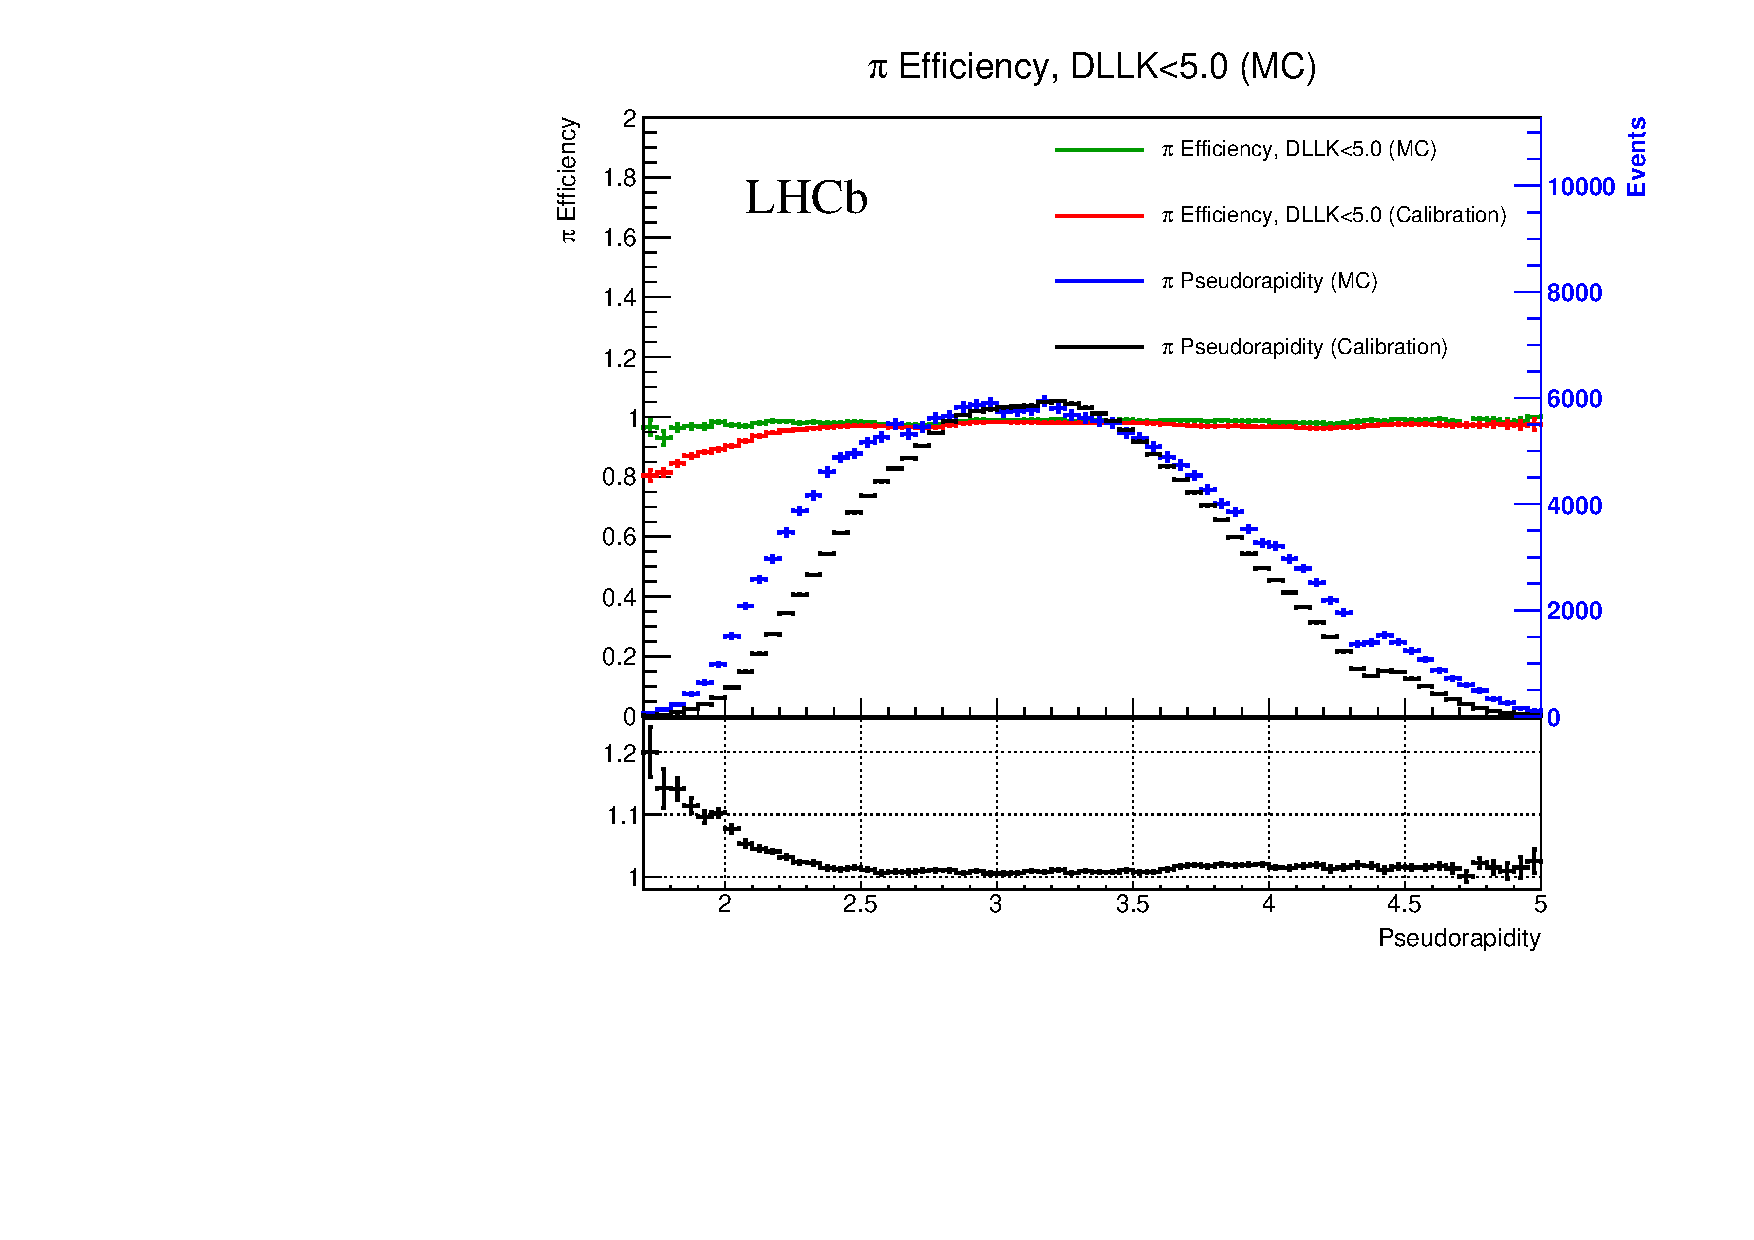
\includegraphics[width=0.495\linewidth]{AA-Appdx-pid/figs/Bd2DPi_BacPi_DLLKlt5_PIDeff_beforeResampling_ETA.pdf} \\
		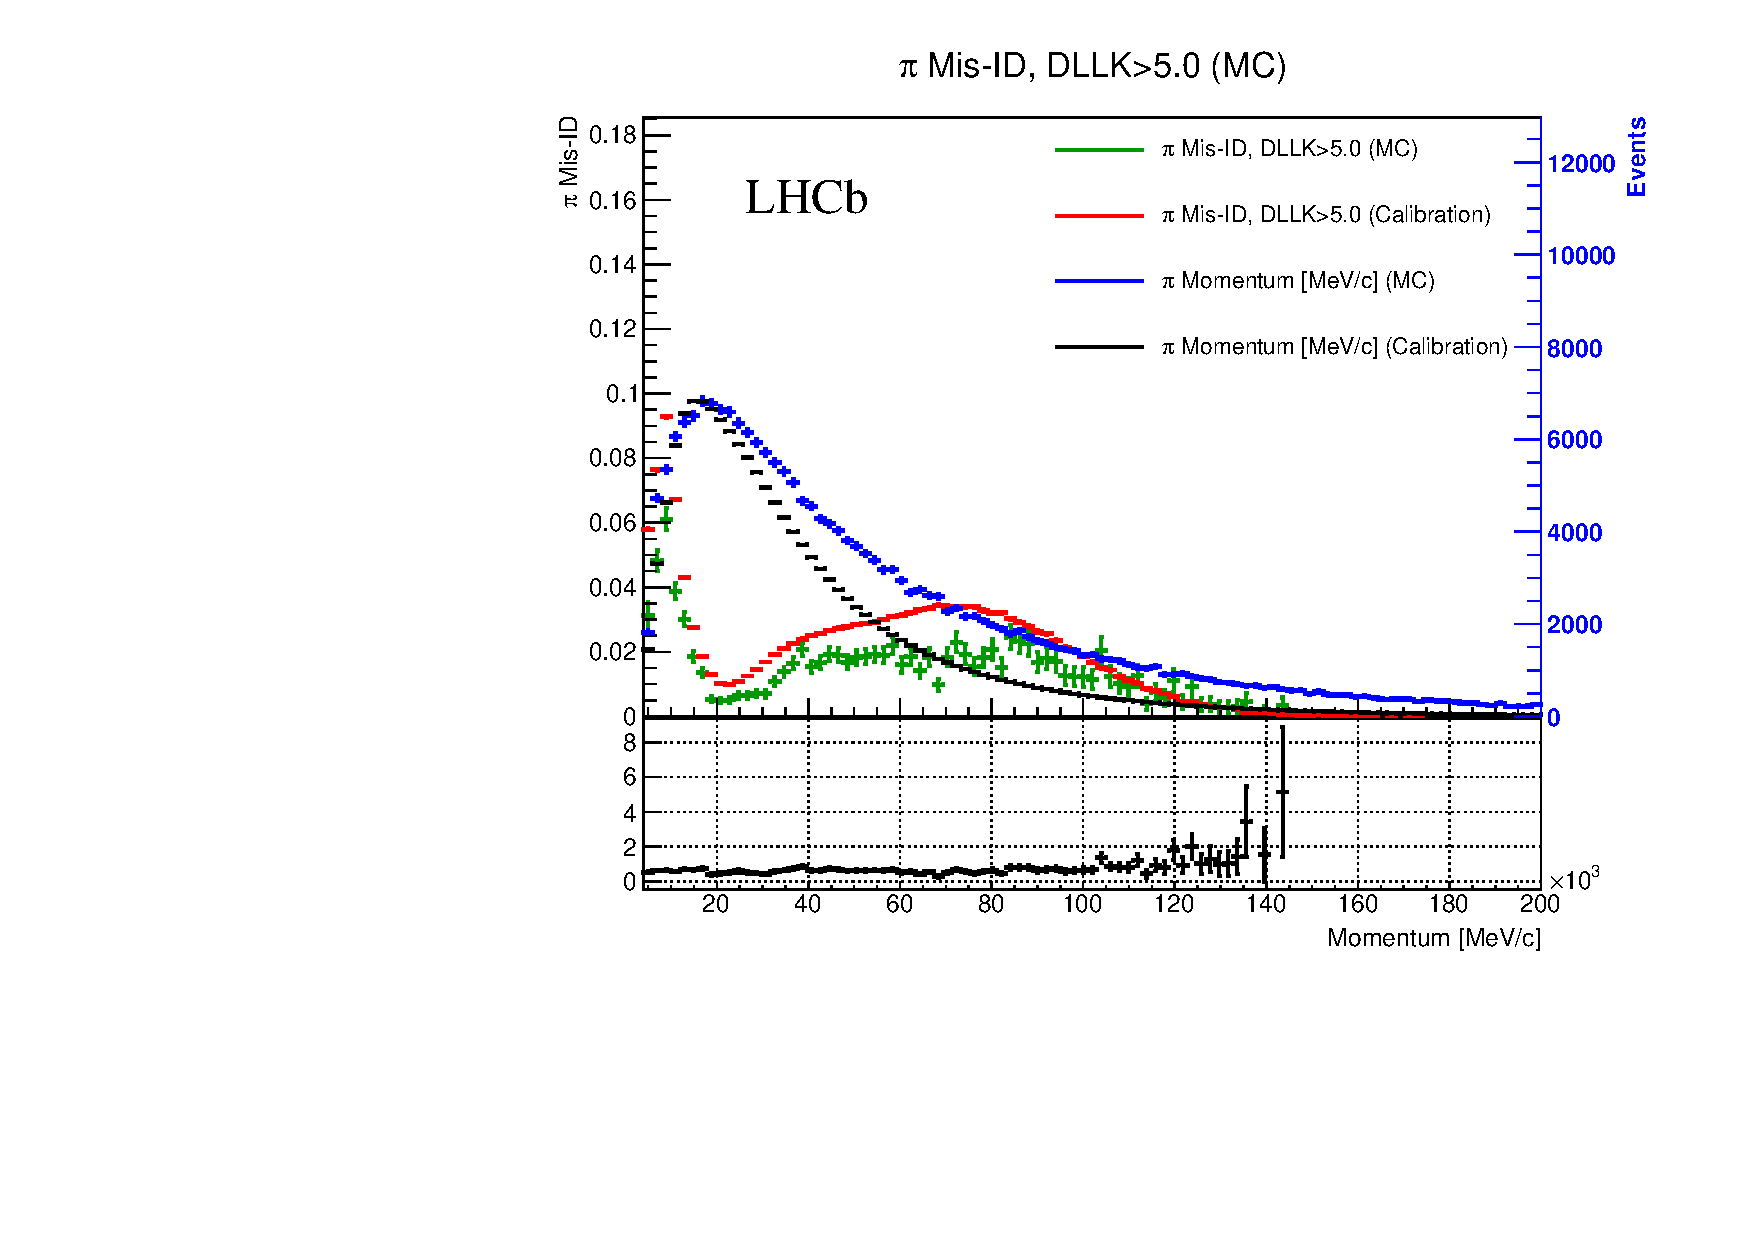
\includegraphics[width=0.495\linewidth]{AA-Appdx-pid/figs/Bd2DPi_BacPi_DLLKgt5_PIDmisID_beforeResampling_P.pdf}
		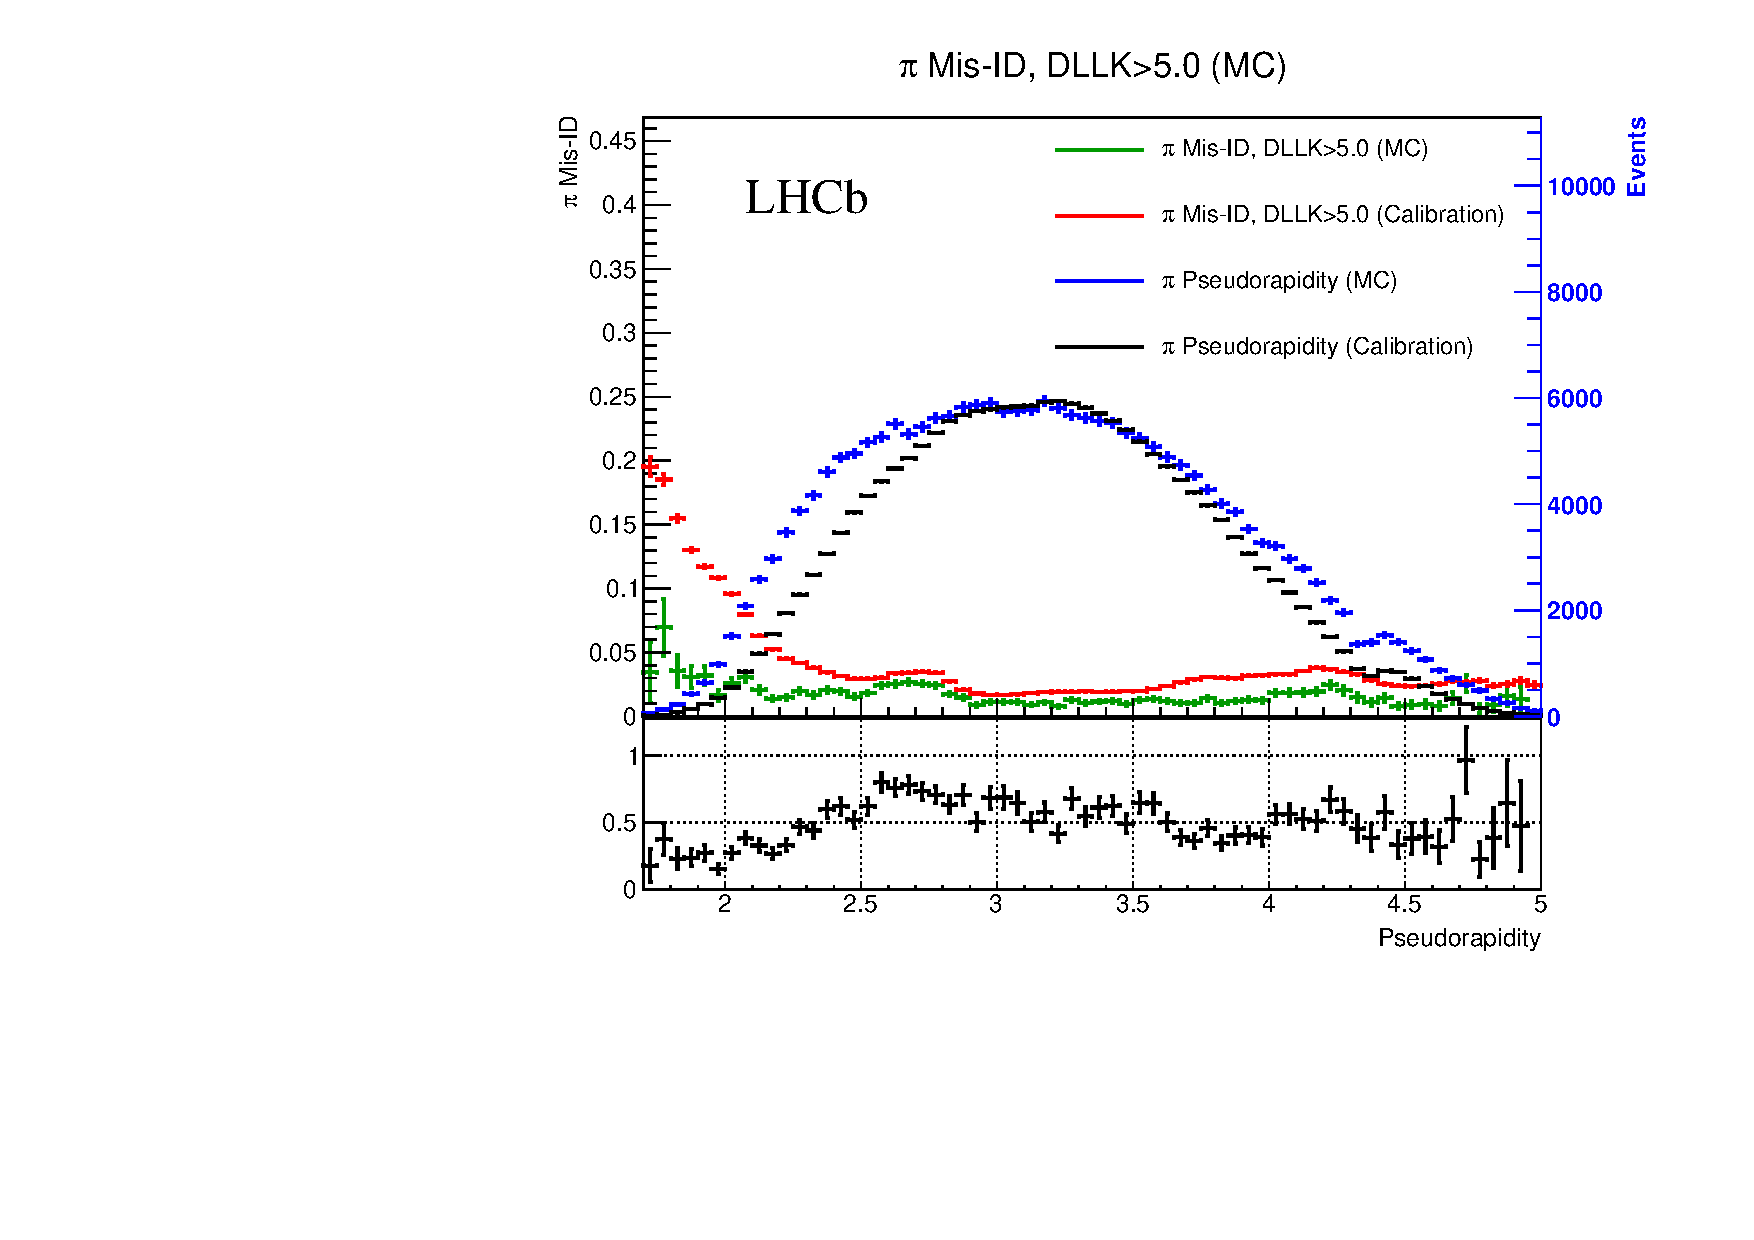
\includegraphics[width=0.495\linewidth]{AA-Appdx-pid/figs/Bd2DPi_BacPi_DLLKgt5_PIDmisID_beforeResampling_ETA.pdf} \\
	\end{center}
        \vspace{-2mm}
	\caption{Efficiencies of the requirements PID$K<5$ (top) and PID$K>5$ (bottom) for bachelor pions as a function of momentum $p$
	(left) and pseudorapidity $\eta$ (right), both for $\Bz\to\Dmp\pipm$ signal MC (green) and calibration mode (red).
	 The superimposed histograms show the $p$ and $\eta$ distributions of the MC signal (blue) and calibration (black) samples.
	The ratio of the
	efficiency or misidentification rate between the MC signal and data calibration
	samples is shown in the lower pad (black).}
	\label{fig:PIDKeffPiBac}
\end{figure}
\begin{figure}[t]
	\begin{center}
		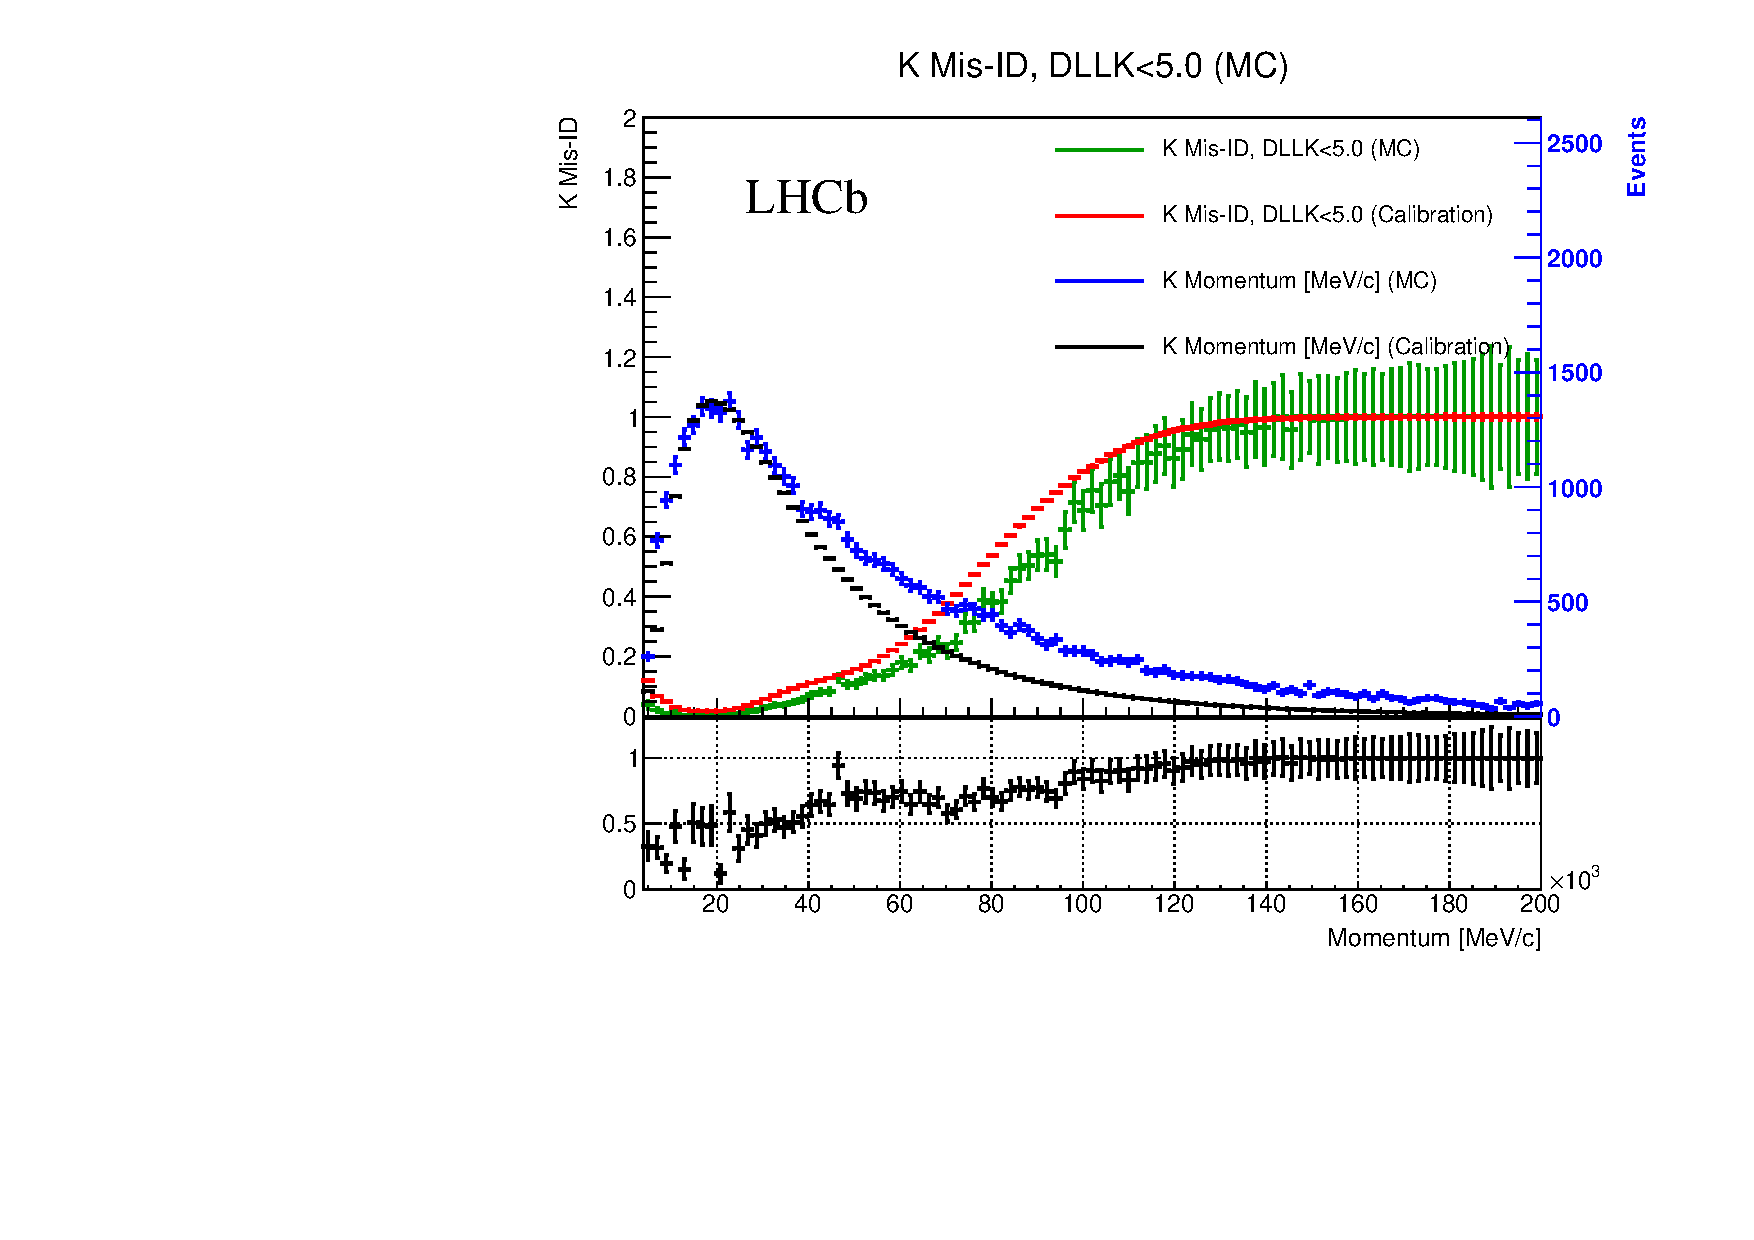
\includegraphics[width=0.495\linewidth]{AA-Appdx-pid/figs/Bd2DK_BacK_DLLKlt5_PIDmisID_beforeResampling_P.pdf}
		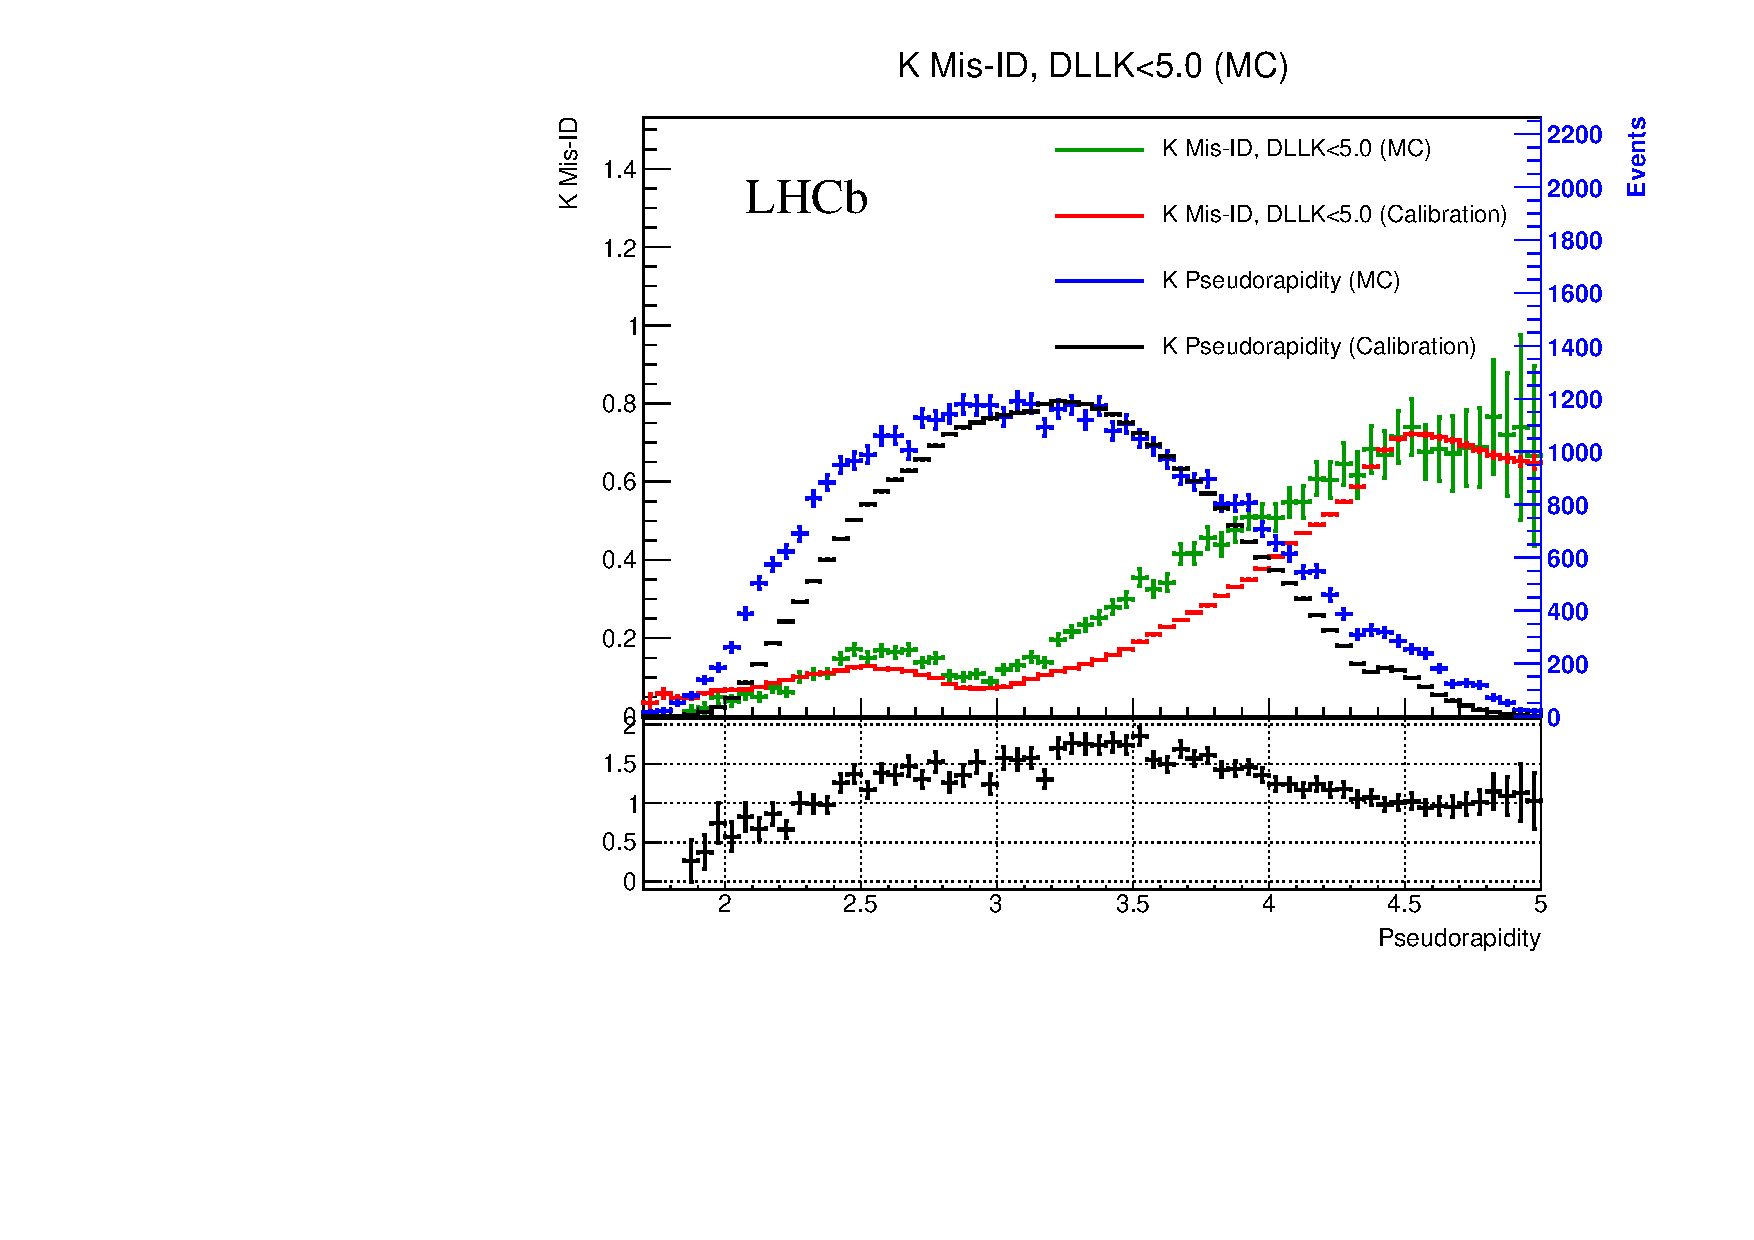
\includegraphics[width=0.495\linewidth]{AA-Appdx-pid/figs/Bd2DK_BacK_DLLKlt5_PIDmisID_beforeResampling_ETA.pdf} \\
		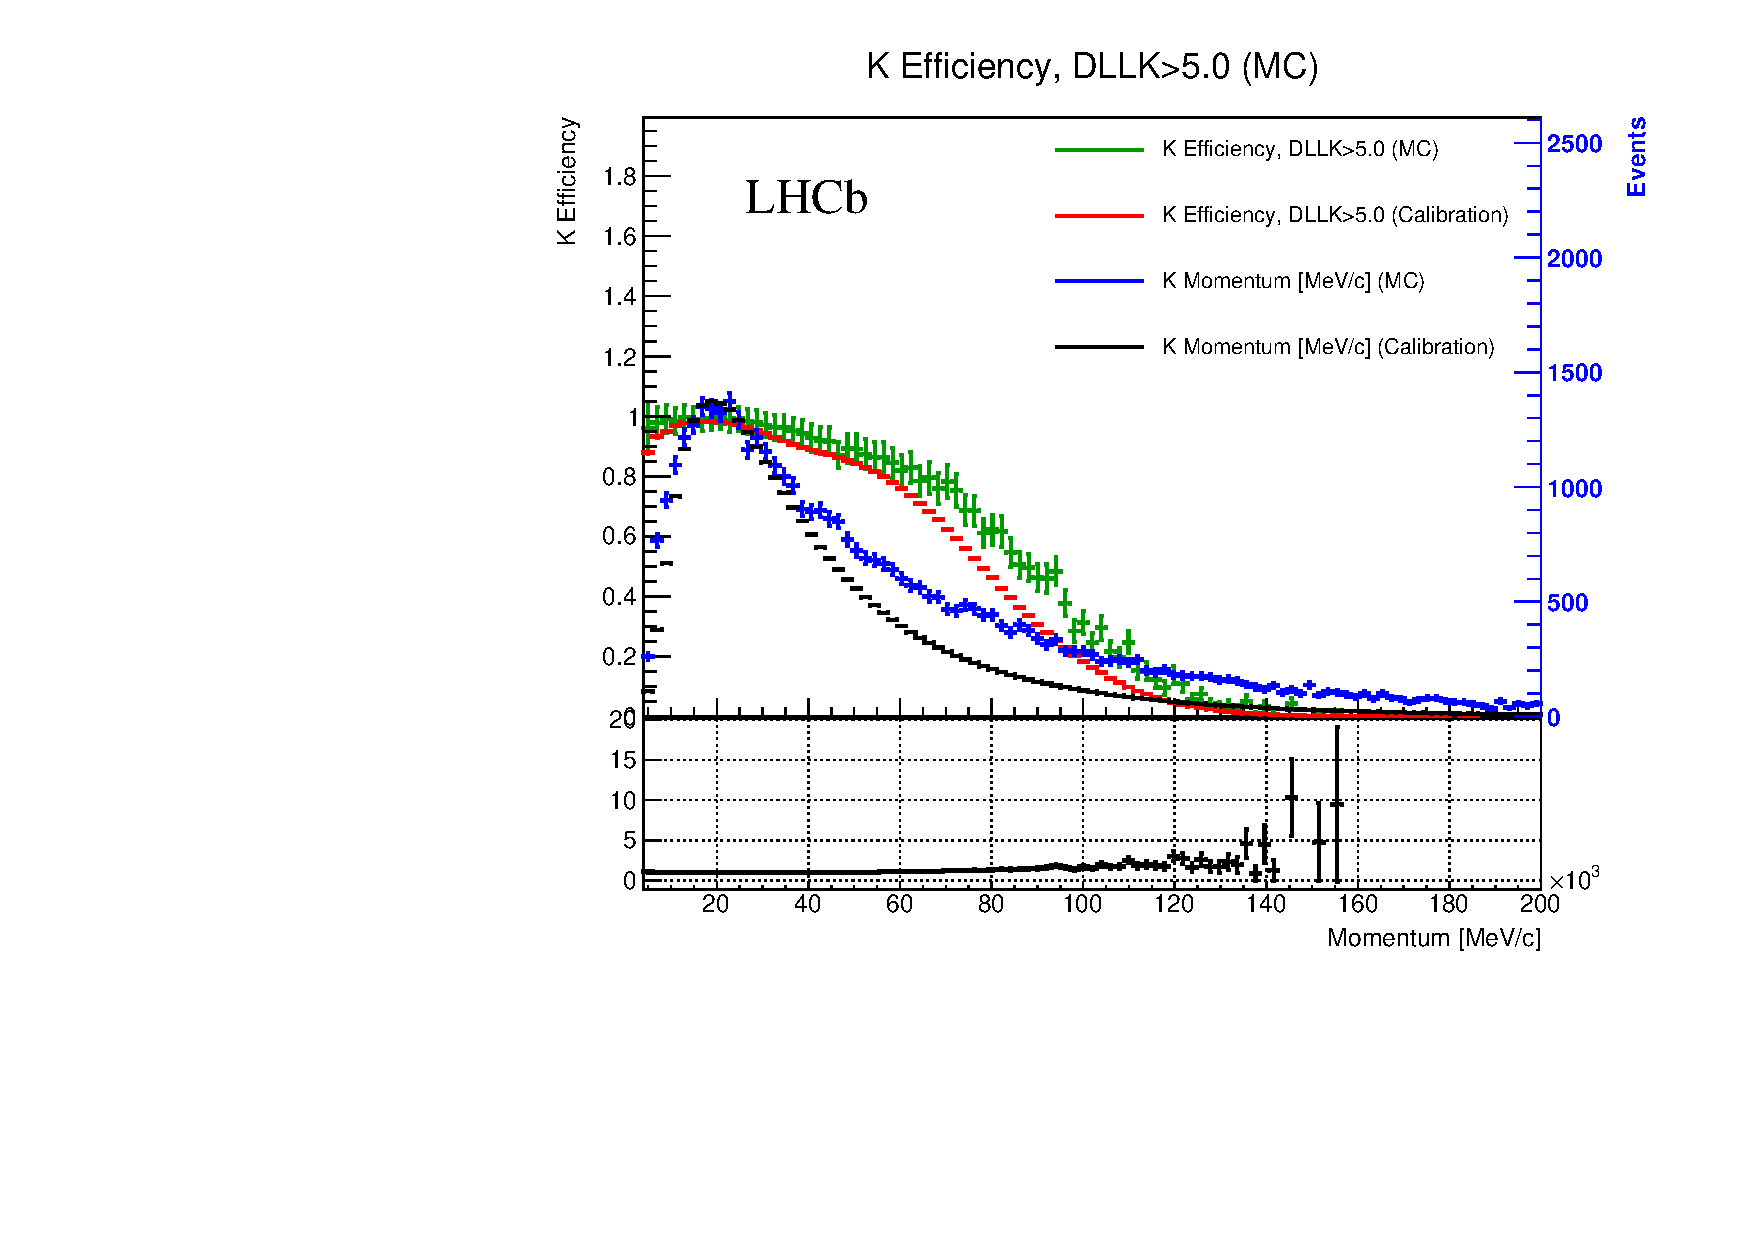
\includegraphics[width=0.495\linewidth]{AA-Appdx-pid/figs/Bd2DK_BacK_DLLKgt5_PIDeff_beforeResampling_P.pdf}
		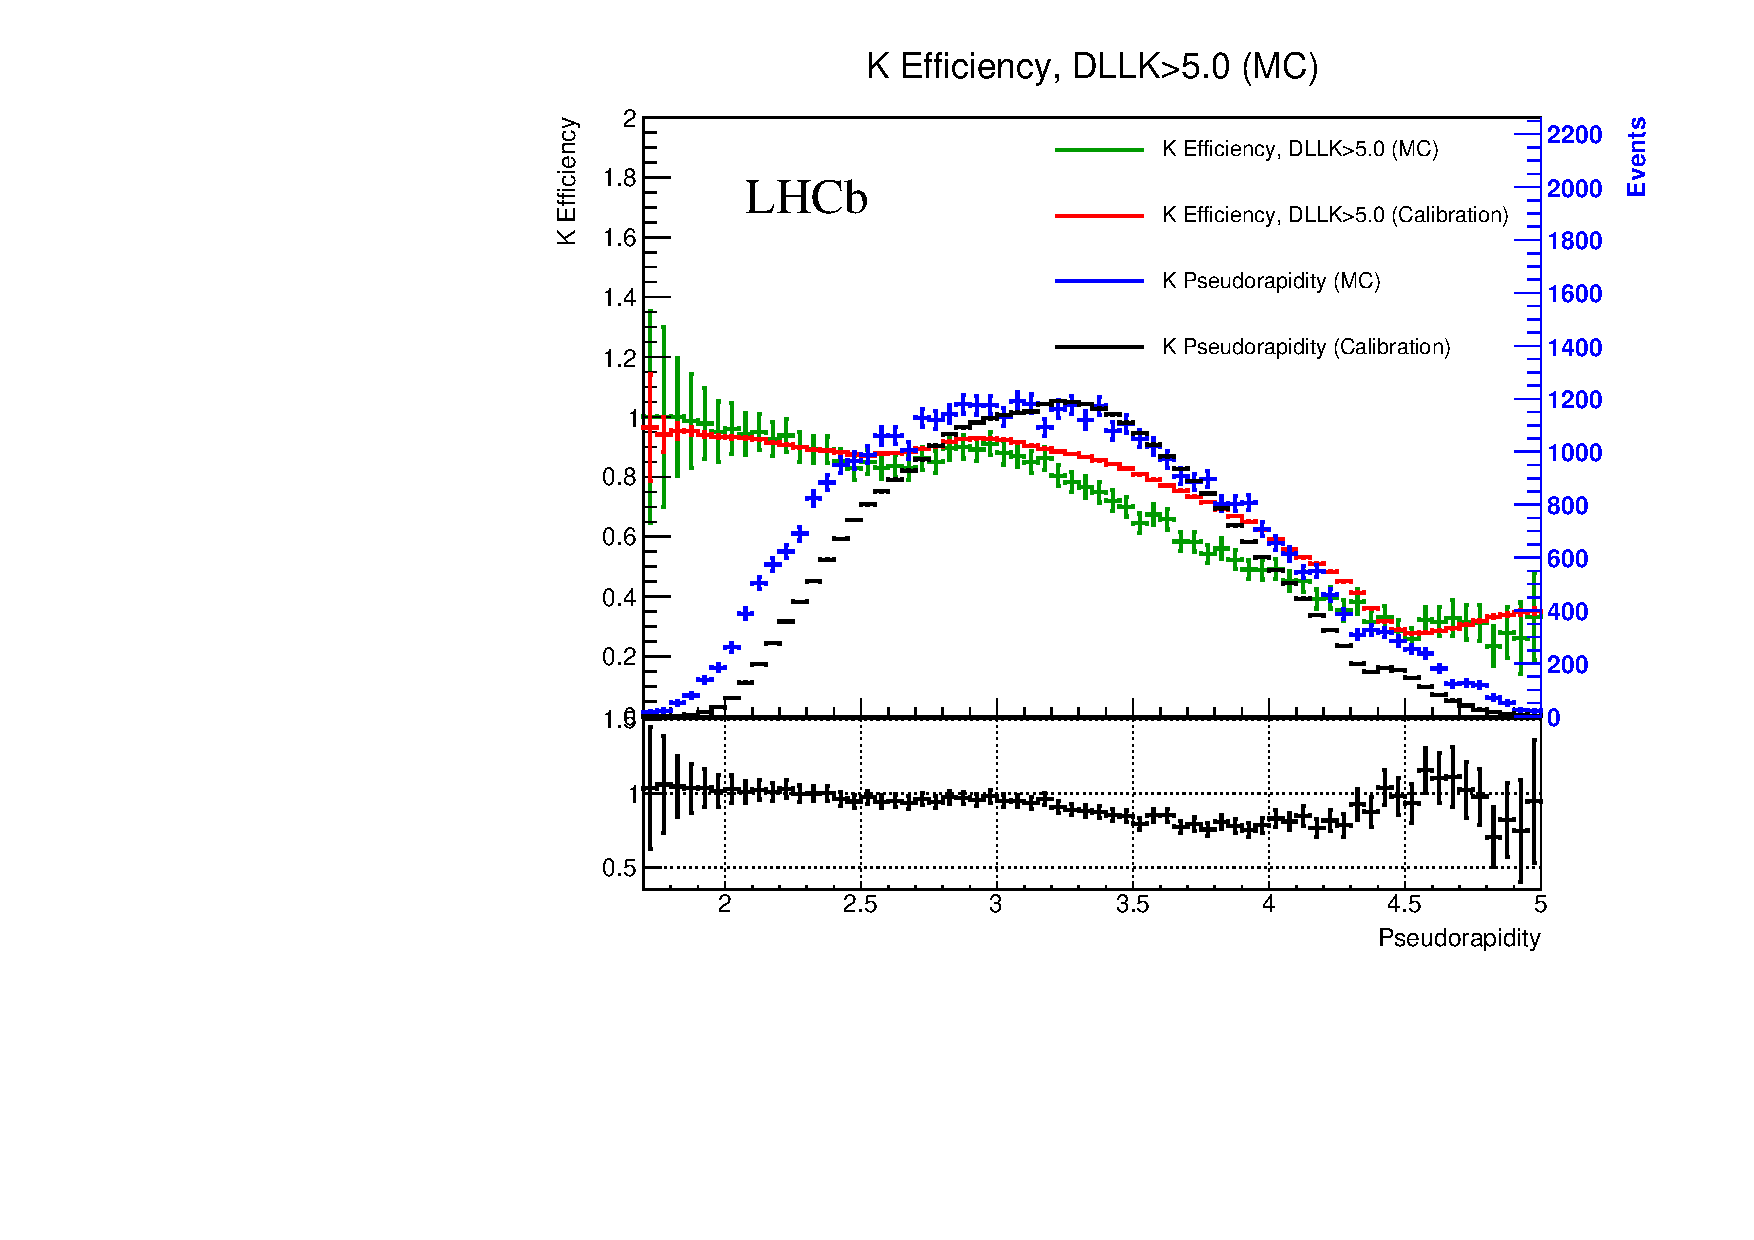
\includegraphics[width=0.495\linewidth]{AA-Appdx-pid/figs/Bd2DK_BacK_DLLKgt5_PIDeff_beforeResampling_ETA.pdf} \\
	\end{center}
        \vspace{-2mm}
	\caption{Efficiencies of the requirements PID$K<5$ (top) and PID$K>5$ (bottom) for bachelor kaons as a function of momentum $p$
	(left) and pseudorapidity $\eta$ (right), both for $\Bz\to\Dmp\Kpm$ MC (green) and calibration mode (red).
	 The superimposed histograms show the $p$ and $\eta$ distributions of the $\Bz\to\Dmp\Kpm$ MC (blue) and calibration (black) samples.
	The ratio of the
	efficiency or misidentification rate between the MC signal and data calibration
	samples is shown in the lower pad (black).}
	\label{fig:PIDKeffKBac}
\end{figure}
\begin{figure}[t]
  \begin{center}
    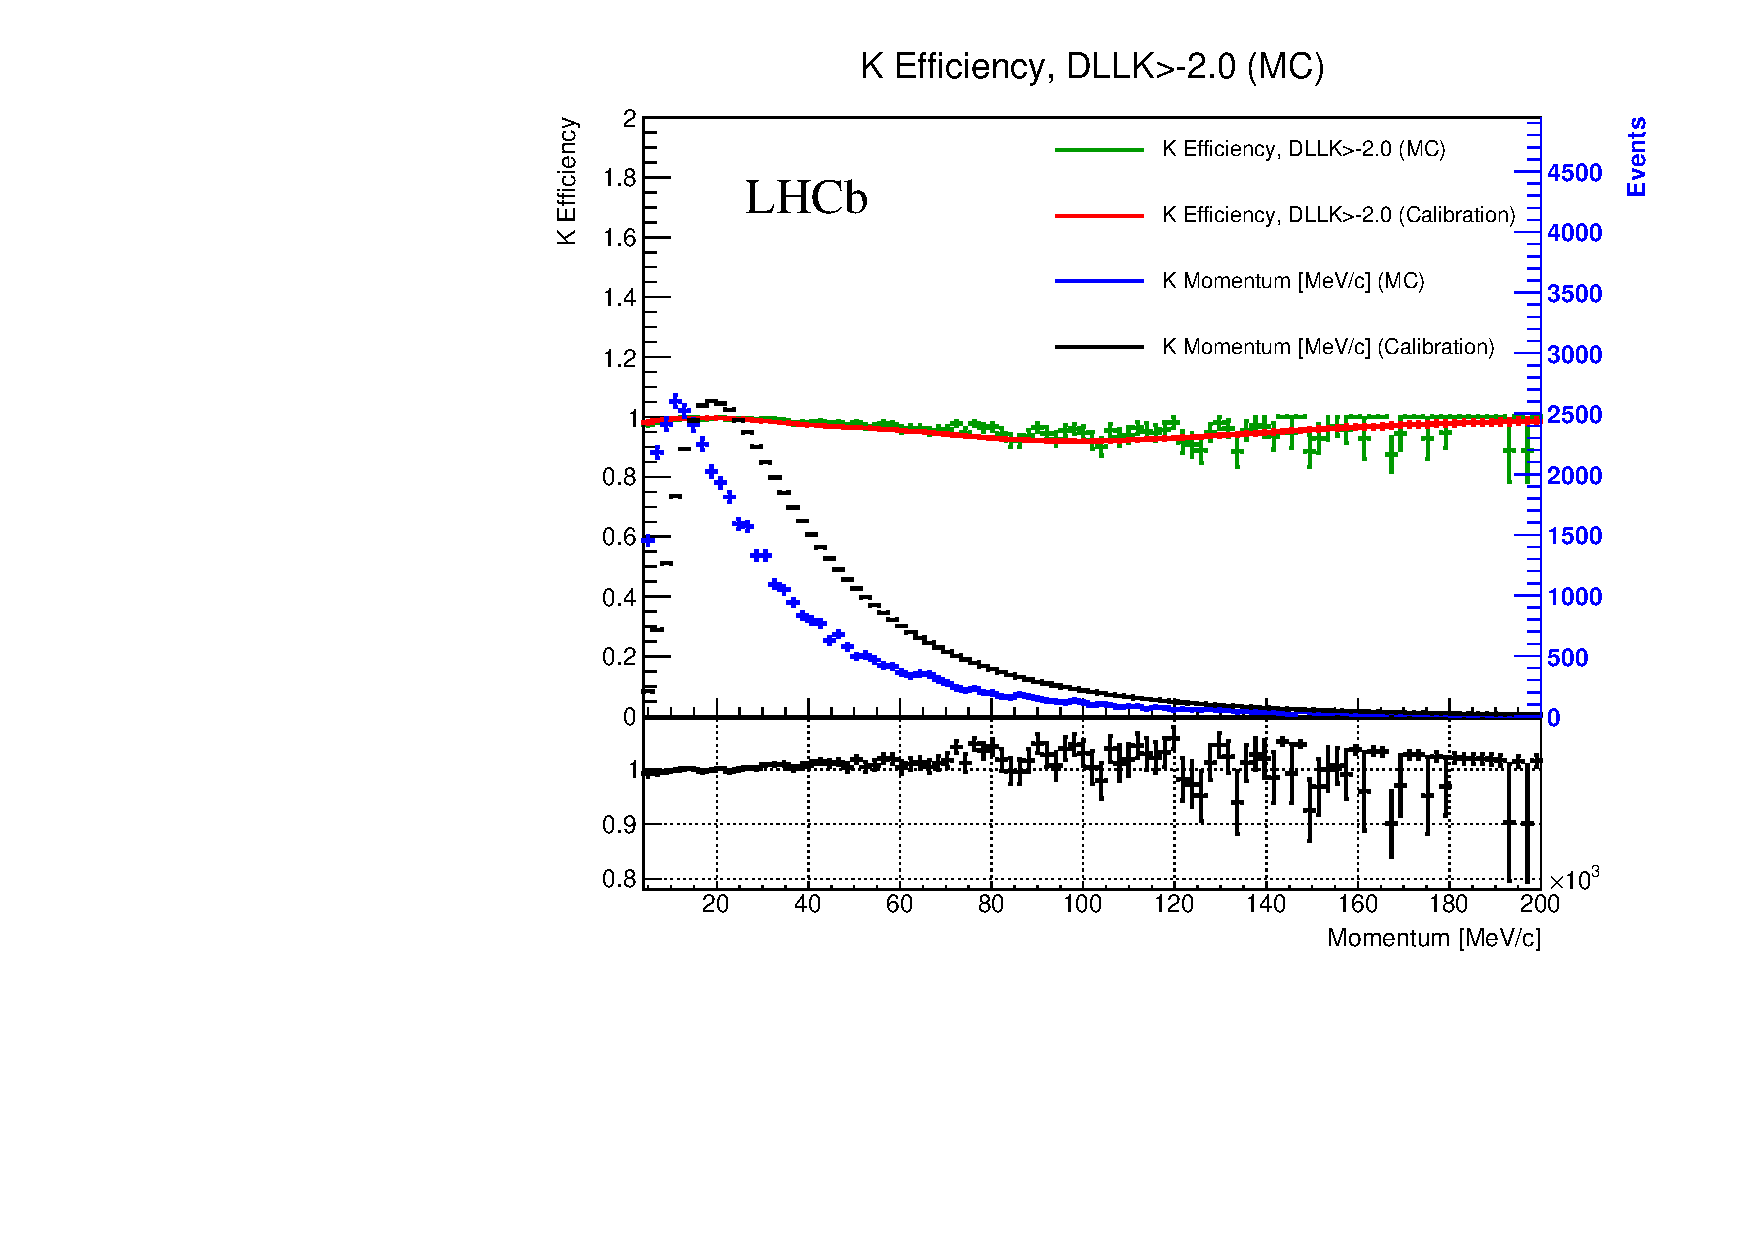
\includegraphics[width=0.495\linewidth]{AA-Appdx-pid/figs/Bd2DPi_KfromD_DLLKgtm2_PIDeff_beforeResampling_P.pdf}
    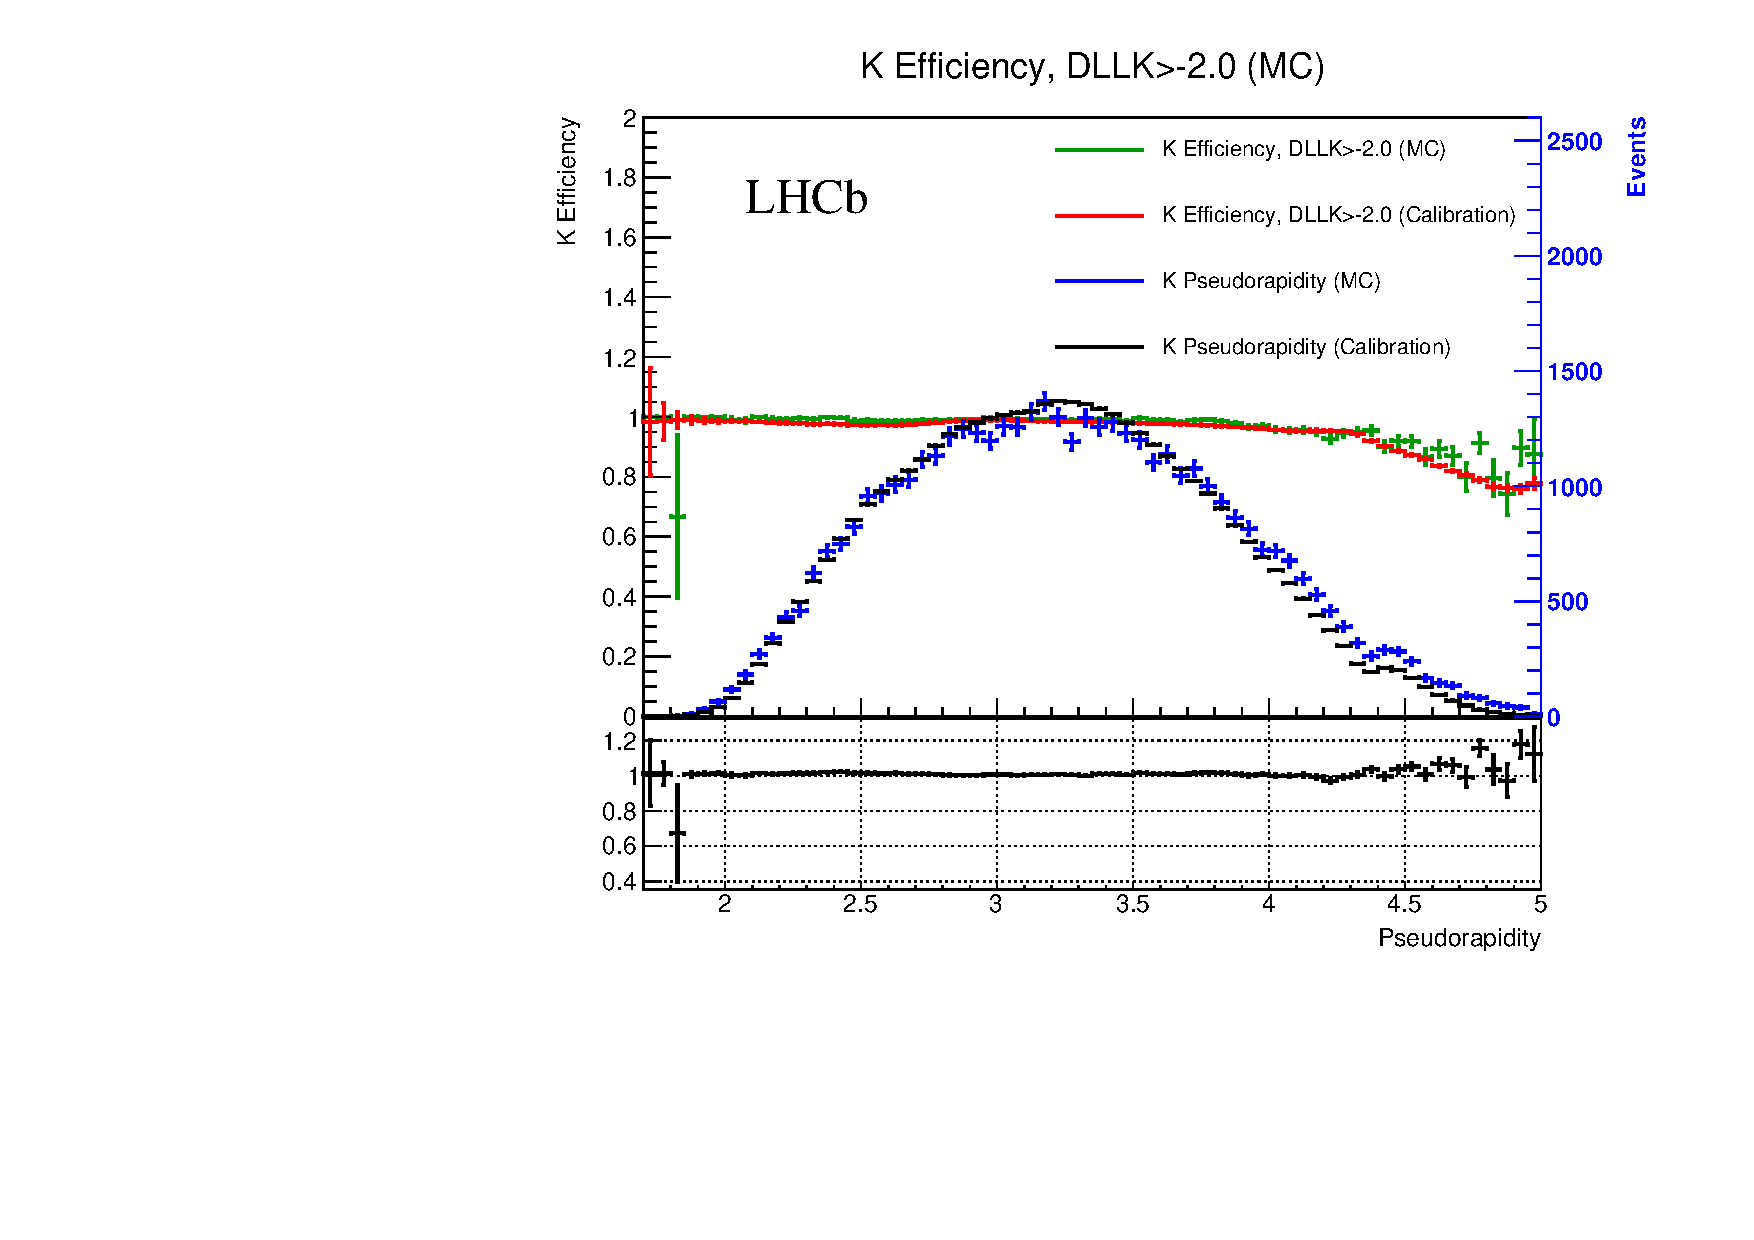
\includegraphics[width=0.495\linewidth]{AA-Appdx-pid/figs/Bd2DPi_KfromD_DLLKgtm2_PIDeff_beforeResampling_ETA.pdf} \\
    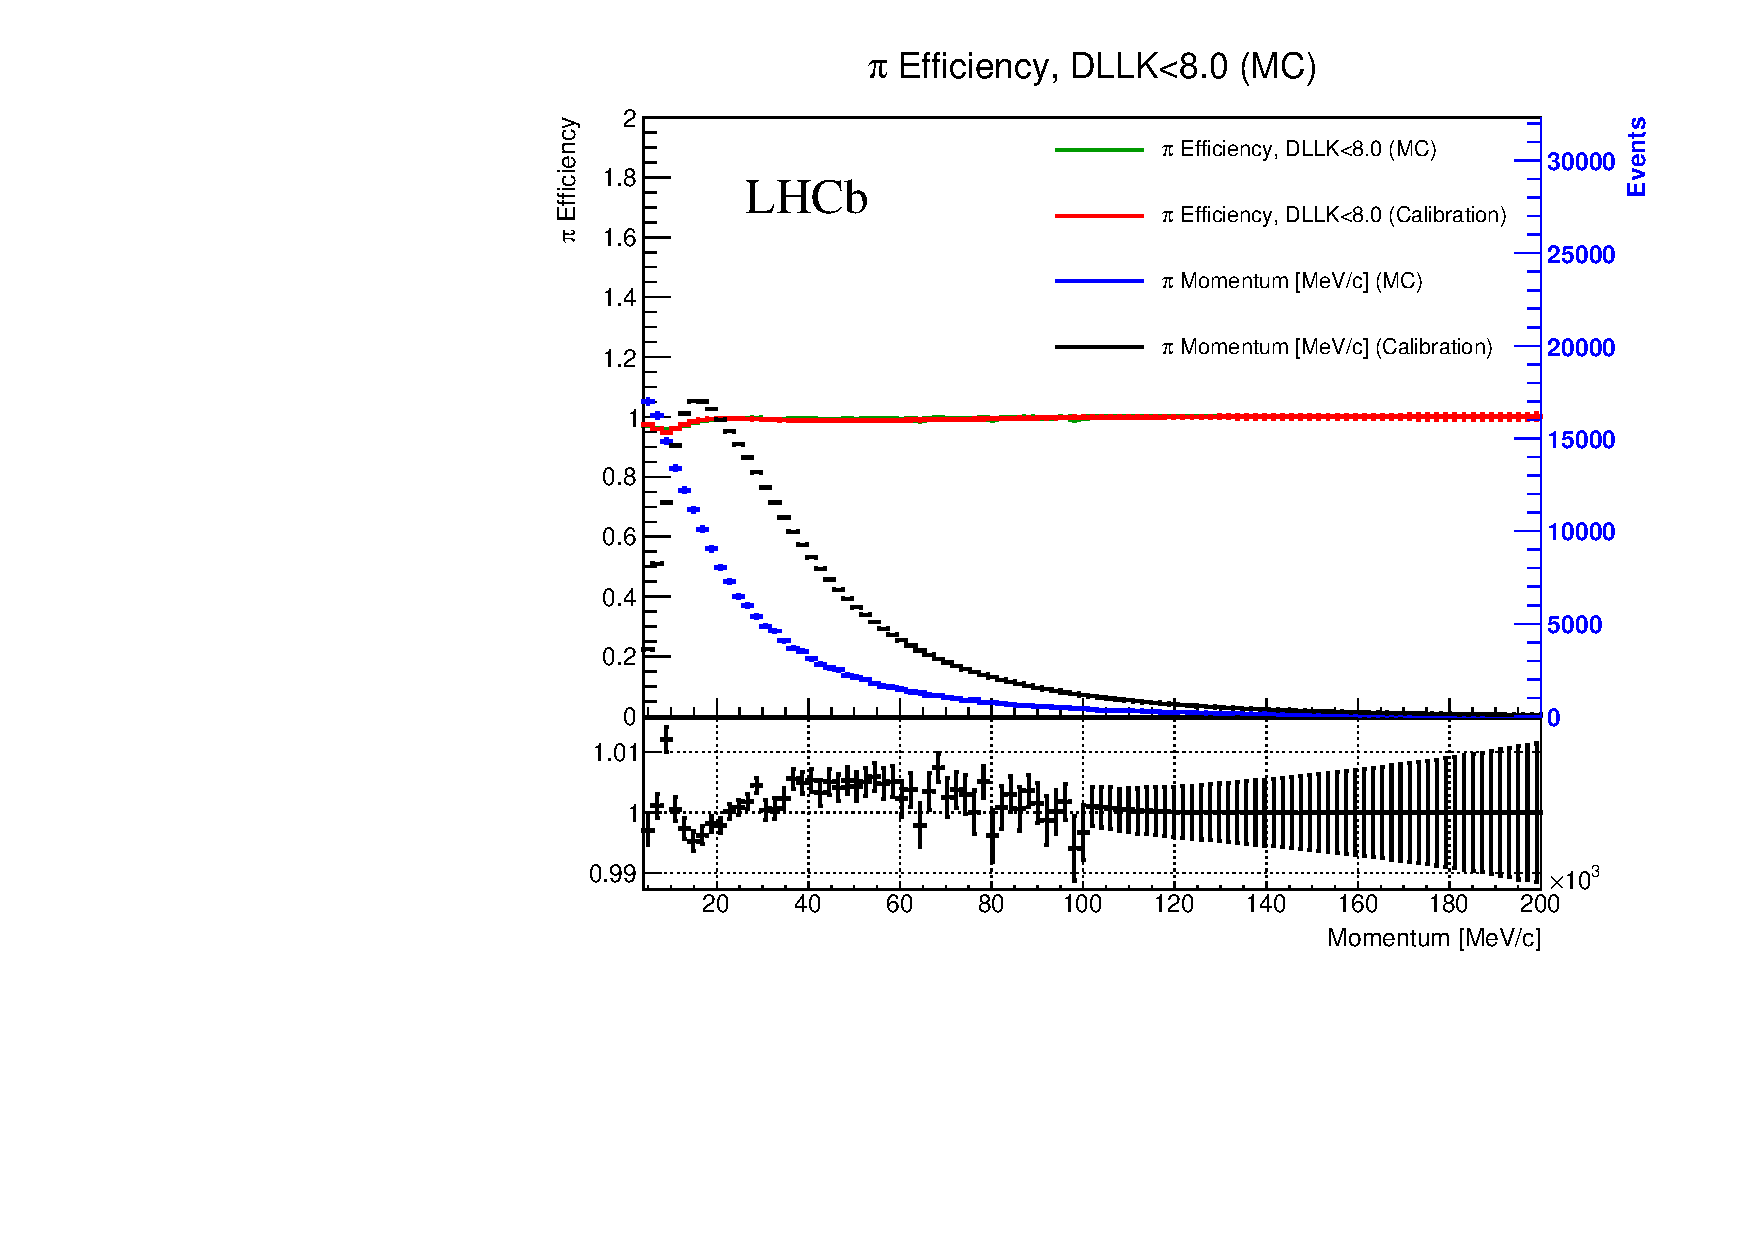
\includegraphics[width=0.495\linewidth]{AA-Appdx-pid/figs/Bd2DPi_Pi1fromD_DLLKlt8_PIDeff_beforeResampling_P.pdf}
    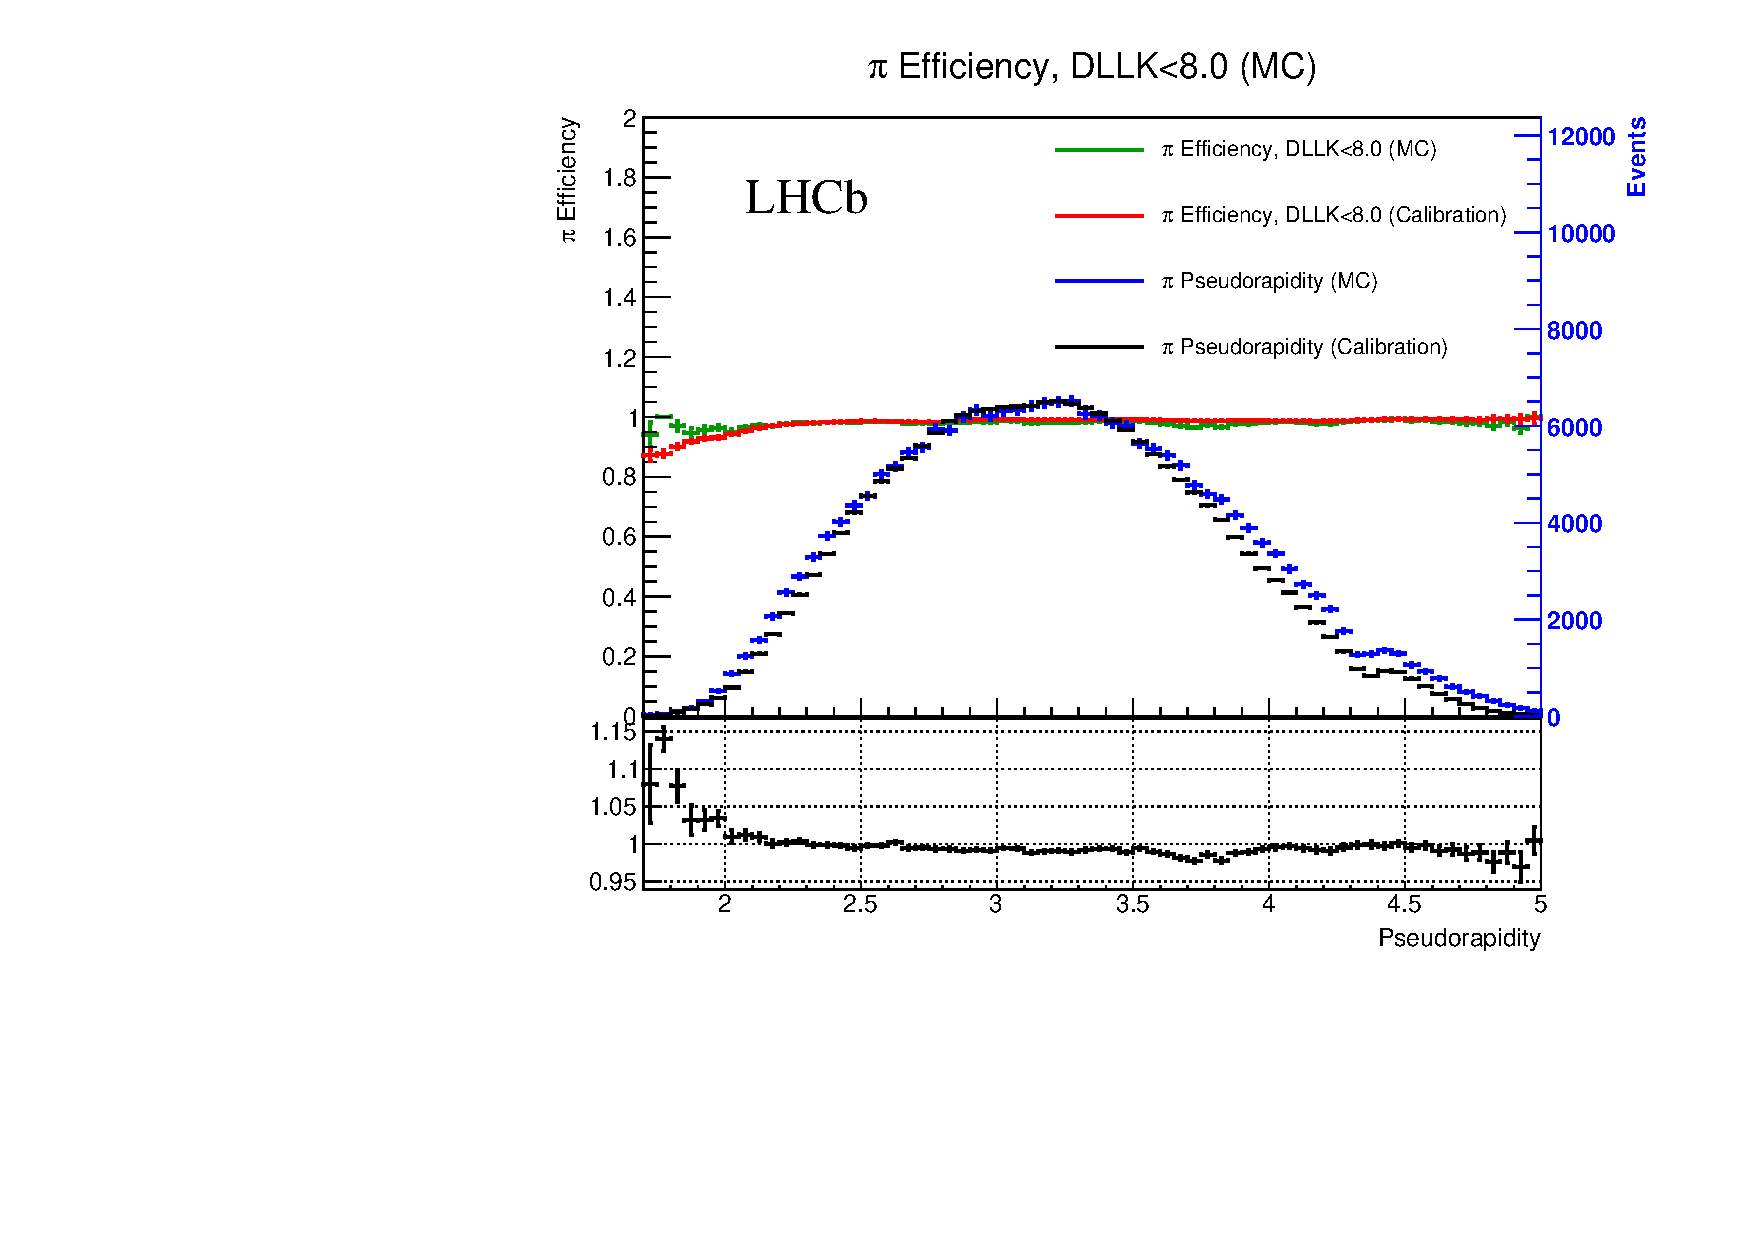
\includegraphics[width=0.495\linewidth]{AA-Appdx-pid/figs/Bd2DPi_Pi1fromD_DLLKlt8_PIDeff_beforeResampling_ETA.pdf} \\
    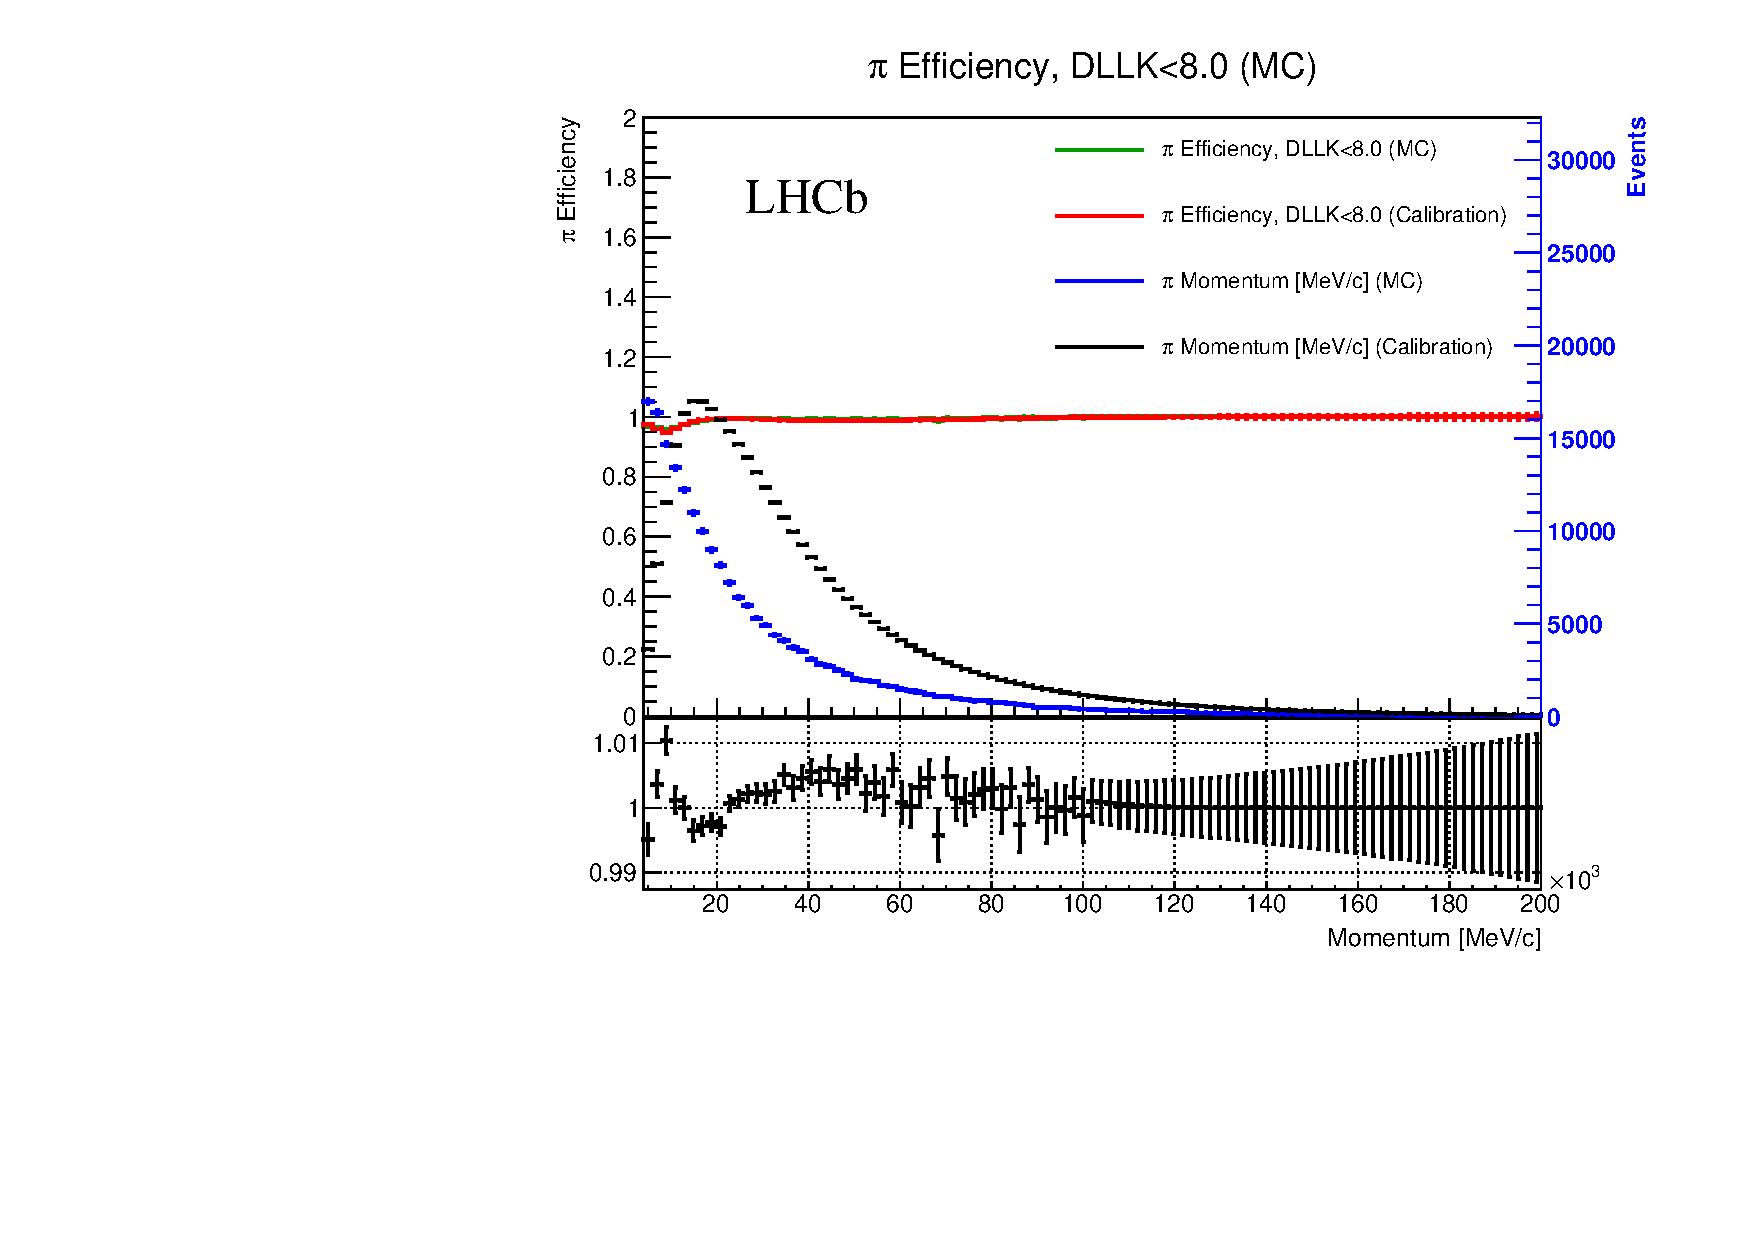
\includegraphics[width=0.495\linewidth]{AA-Appdx-pid/figs/Bd2DPi_Pi2fromD_DLLKlt8_PIDeff_beforeResampling_P.pdf}
    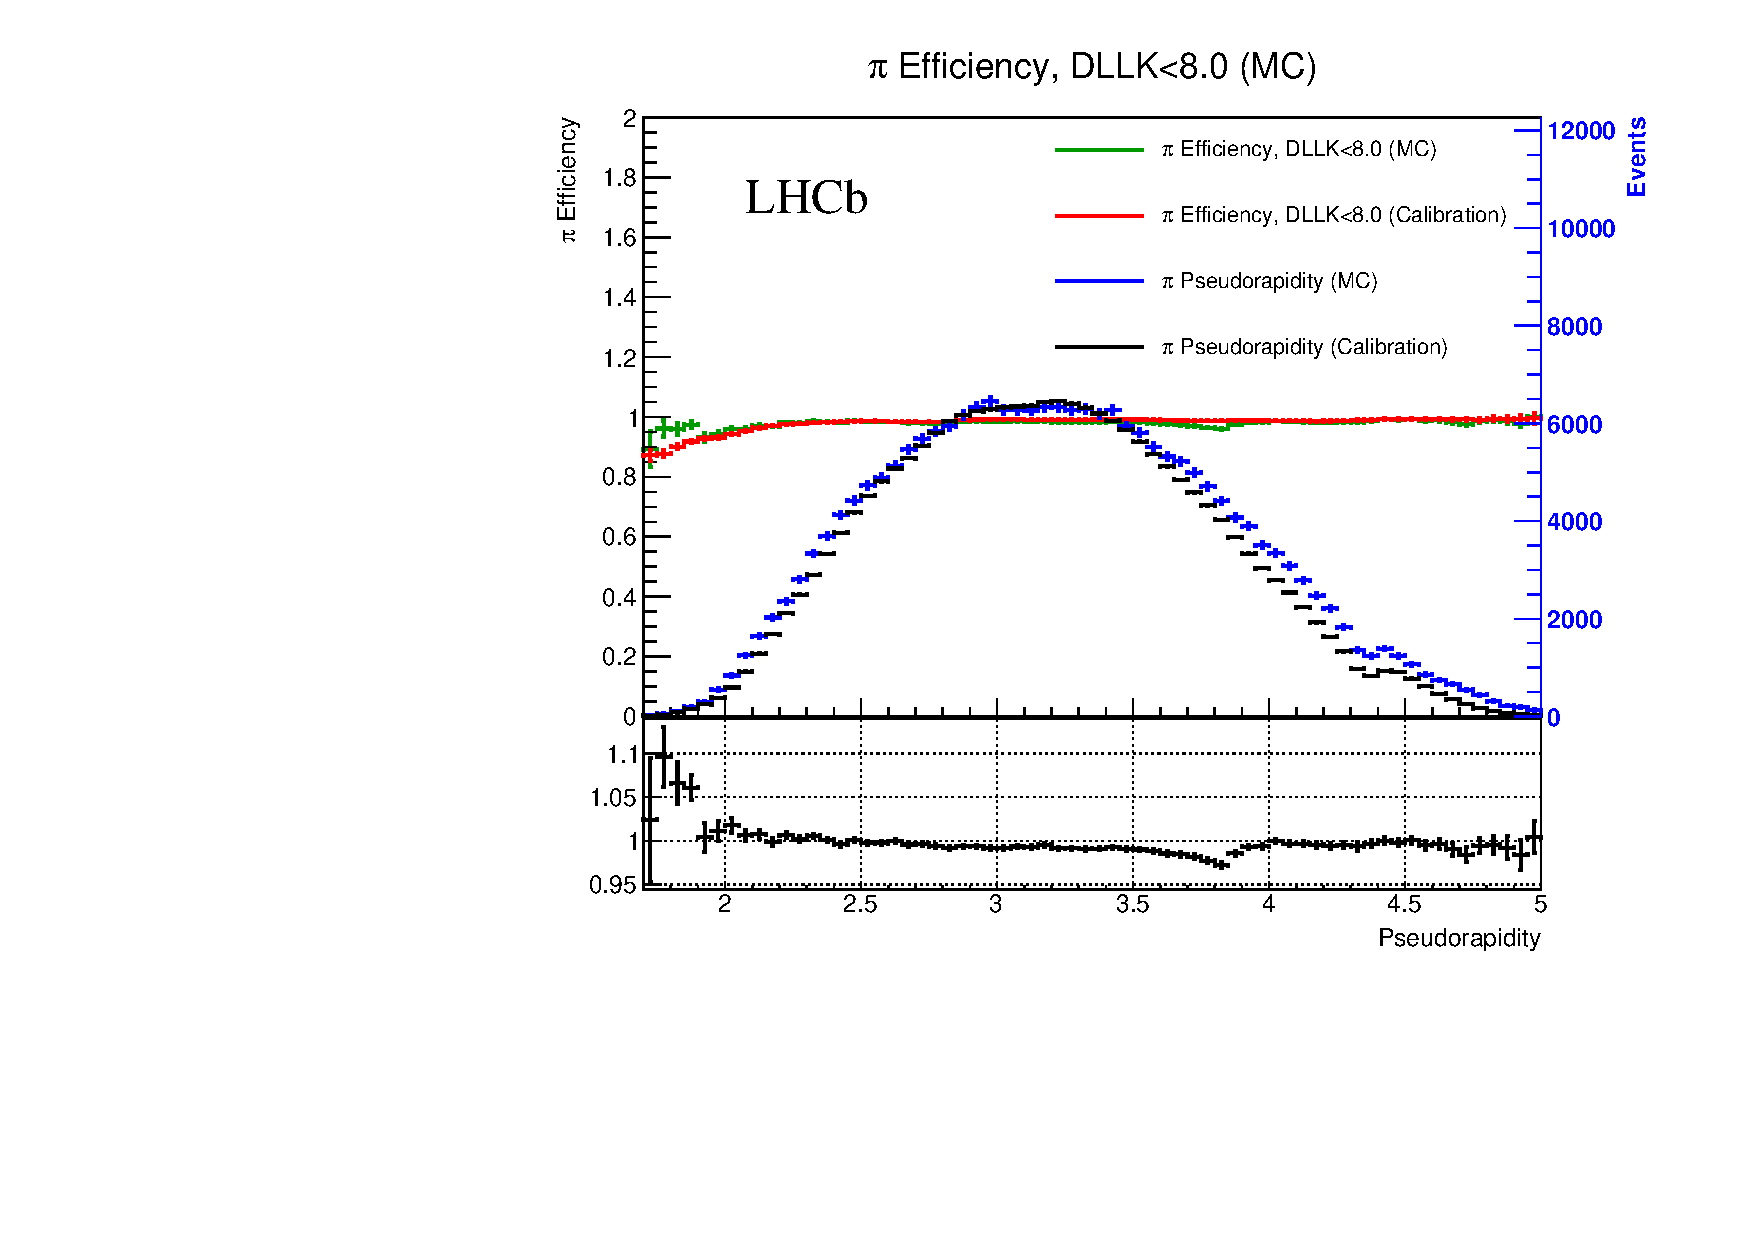
\includegraphics[width=0.495\linewidth]{AA-Appdx-pid/figs/Bd2DPi_Pi2fromD_DLLKlt8_PIDeff_beforeResampling_ETA.pdf}
  \end{center}
  \vspace{-2mm}
  \caption{$\PIDK$ efficiencies for the kaon (top) and the two pions (middle, bottom) produced in the $\Dmp$ decay as a function of momentum $p$
	(left) and pseudorapidity $\eta$ (right), both for $\Bz\to\Dmp\pipm$ signal MC (green) and calibration mode (red).
	 The superimposed histograms show the $p$ and $\eta$ distributions of the MC signal (blue) and calibration (black) samples.
	The ratio of the
	efficiency between the MC signal and data calibration
	samples is shown in the lower pad (black).}
  \label{fig:PIDKeffBac}
\end{figure}
